\section{Spatial discretization along homogeneous directions}
Our solver is based on a Fourier approach. Among the advantages of such approach we face the possibility to expansion of the unknown functions in terms of truncated Fourier series in the homogeneous directions. For example the wall-normal component $v$ of the velocity vector is represented as:
\begin{equation}
v(x,y,z,t) = \sum_{h=-nx/2}^{+nx/2} \sum_{l=-nz/2}^{+nz/2} \hat{v}_{hl}(y,t) e^{i\alpha x}e^{i \beta z}
\end{equation}
where:
\begin{equation}
\alpha = \frac{2\pi h}{L_{x}} = \alpha_{0} h; \quad \beta= \frac{2 \pi l}{L_{z}} = \beta_{0}l
\end{equation}

$h$ and $l$ are integer indexes corresponding to the streamwise and spanwise direction respectively, and $\alpha_{0}$ and $\beta_{0}$ are the fundamental wavenumbers in these directions, defined in terms of the streamwise and spanwise lengths $L_{x} = {2\pi}/{\alpha_{0}} $ and $L_{z} = {2 \pi}/{\beta_{0}}$ of the computational domain. The computational parameters given by the streamwise and spanwise lenght of the computational domain, $L_{x}$ and $L_{z}$ , and the truncation of the series, $nx$ and $nz$, must be chosen so as to miminize computational errors. For further details regarding the proper choice of a value of $L_{x}$ see~\cite{QuadrioMaurizio2003Issi}.

The convolutions required to solve the equations~\ref{curl:momentum:y} and~\ref{normal:velocity} are computationally expensive if carried out in the frequency domain. The same evaluation can be performed efficiently by first transforming the three Fourier components of velocity back in physical space, multiplying them in all six possible pair combinations and eventually retransforming the results into the Fourier space. Fast Fourier Transform algorithms are used to move from Fourier to physical space and viceversa. The aliasing error is removed by expanding the number of modes by a factor of at least $3/2$ before the inverse Fourier transforms, to avoid the introduction of spurious energy from the high-frequency into the low-frequency modes during the calculation~\cite{ns:quadrio}.





\section{Finite difference scheme}
The discretization of the wall-normal derivatives $D_{1}$, $D_{2}$ and $D_{4}$, required for the numerical solution of the present problem, is performed through finite difference (FD) compact schemes~\cite{finite:difference:scheme} with fourth-order accuracy over a computational molecule composed by five arbitrarily spaced grid points. We indicate here with $d_{1}^{j} (i), i = -2, \dots , 2$ the five coefficients discretizing the exact operator $D_{1}$ over five adjacent grid points centered at $y_{j}$ :
\begin{equation}
D_{1} \big( f(y) \big) \vert_{y=y_{j}} = \sum_{i=-2}^{2} d_{1}^{j} (i) f(y_{j+i})
\end{equation}
The basic idea of compact schemes can be most easily understood by thinking of a standard FD formula in Fourier space as a polynomial interpolation of a trascendent function, with the degree of the polynomial corresponding to the formal order of accuracy of the FD formula. Compact schemes improve the interpolation by replacing the polynomial with a ratio of two polynomials, i.e. with a rational function. This obviously increases the number of available coefficients, and moreover gives control over the behavior at infinity (in frequency space) of the interpolant, whereas a polynomial necessarily diverges. This allows a compact FD formula to approximate a differential operator in a wider frequency range, thus achieving resolution properties similar to those of spectral schemes~\cite{finite:difference:scheme}.
Compact schemes are also known as implicit finite-differences schemes, because they typically require the inversion of a linear system for the actual calculation of a derivative~\cite{compact:difference}\cite{finite:difference:scheme}.
 Here we are able to use compact, fourth-order accurate schemes at the cost of explicit schemes, owing to the absence of the third-derivative operator from the equations of motion. Thanks to this property, it is possible to find rational function approximations for the required three FD operators, where the denominator of the function is always the same, as highlighted first in the original Gauss-Jackson-Noumerov compact formulation exploited in his seminal work by Thomas~\cite{Thomas:coeff}, concerning the numerical solution of the Orr-Sommerfeld equations.\par
To illustrate Thomas’ method, let us consider an 4th-order one-dimensional ordinary differential equation, linear for simplicity, in the form:
\begin{equation}
D_{4}(a_{4}f) + D_{2}(a_{2}f)+D_{1}(a_{1}f)+a_{0}f = g,
\label{Thomas:coeff}
\end{equation}
Where the coefficients $a_{i}= a_{i}(y)$ are arbitrary functions of the independent variable $y$, and $g = g(y)$ is a known RHS. Let us moreover suppose that a differential operator, for example $D_{4}$, is approximated in frequency space as the ratio of two polynomials, say $\mathcal{D}_{4}$ and $\mathcal{D}_{0}$. Polynomials like $\mathcal{D}_{4}$ and $\mathcal{D}_{0}$ have their counterpart in physical space, and ${d}_{4}$ and $d_{0}$ are the corresponding FD operators. The key point is to impose that all the differential operators appearing in the example equation~\ref{Thomas:coeff} admit a representation such as the preceding one, in which the polynomial $\mathcal{D}_{0}$ at the denominator remains the same.\par
Equation~\ref{Thomas:coeff} can thus be recast in the new, discretized form:
\begin{equation}
d_{4} (a_{4}f) + d_{2} (a_{3}f) + d_{1} (a_{1}f) + d_{0} (a_{0}f) = d_{0} g,
\end{equation}
and this allows us to use explicit FD formulas, provided the operator $d_{0}$ is applied to the right-hand-side of our equations. The overhead related to the use of implicit finite difference schemes disappears, while the advantage of using high-accuracy compact schemes is retained~\cite{ns:quadrio}.





\subsection{Compute of the finite difference coefficients}










\section{Time discretization}
Time integration of the equations is performed by a partially-implicit method.
The use of a partially-implicit scheme is a common approach in DNS~\cite{kim_moin_moser}: the explicit part of the equations can benefit from a higher-accuracy scheme, while the stability-limiting viscous part is subjected to an implicit time advancement, thus relieving the stability constraint on the time-step size $	\Delta t$. \par
Our preferred choice, following~\cite{cpl:presentazione}\cite{kim_moin_moser} is to use an explicit third-order, low-storage Runge-Kutta method for the integration of the explicit part of the equations, and an implicit second-order Crank-Nicolson scheme is used for the implicit part. This scheme has been anyway embedded in a modular coding implementation that allows us to change the time-advancement scheme very easily without otherwise affecting the structure of the code. In fact, we have a few other time-advancement schemes built into the code for testing purposes. \par
 Here we present the time-discretized version of equations~\ref{curl:momentum:y} and~\ref{normal:velocity} for a generic wavenumber pair and a generic two-levels scheme for the explicitly-integrated part coupled with the implicit Crank-Nicolson scheme:
\begin{multline}
\frac{\lambda}{\Delta t} \hat{\eta}_{hl}^{n+1} -\frac{1}{Re} \big[ D_{2} (\hat{\eta}_{hl}^{n+1}) - k^{2} \hat{\eta}_{hl}^{n+1} \big] = \\
\frac{\lambda}{\Delta t} \hat{\eta}_{hl}^{n} + \frac{1}{Re} \big[ D_{2} (\hat{\eta}_{hl}^{n}) - k^{2} \hat{\eta}_{hl}^{n} \big] + \\
\theta \bigg( i\beta_{0}l\widehat{HU}_{hl} - i\alpha_{0}h\widehat{HW}_{hl} \bigg)^{n} + \xi \bigg( i\beta_{0}l\widehat{HU}_{hl} - i\alpha_{0}h \widehat{HW}_{hl} \bigg)^{n-1}
\end{multline}
\begin{multline}
\frac{\lambda}{\Delta t} \big( D_{2} (\hat{v}_{hl}^{n+1}) - k^{2} \hat{v}_{hl}^{n+1} \big) -\frac{1}{Re} \big[ D_{4} (\hat{v}_{hl}^{n+1}) -2 k^{2} D_{2} (\hat{v}_{hl}^{n+1}) + k^{4} \hat{v}_{hl}^{n+1} \big] =\\
\frac{\lambda}{\Delta t} \big( D_{2}(\hat{v}_{hl}^{n}) - k^{2}\hat{v}_{hl}^{n} \big) + \frac{1}{Re} \big[ D_{4} (\hat{v}_{hl}^{n}) -2 k^{2} D_{2} (\hat{v}_{hl}^{n}) + k^{4} \hat{v}_{hl}^{n} \big]+ \\
\theta \bigg( -k^{2} \widehat{HV}_{hl} -D_{1} \big( i\alpha_{0} h \widehat{HU}_{hl} + i\beta_{0} l \widehat{HW}_{hl} \big)  \bigg)^{n} + \\
\xi \bigg( -k^{2} \widehat{HV}_{hl} -D_{1} \big( i\alpha_{0}h\widehat{HU}_{hl} + i\beta_{0}l \widehat{HW}_{hl} \big) \bigg)^{n-1}
\end{multline}

The three coefficients $\lambda$, $\theta$ and $\xi$ define a particular time-advancement scheme. For the simplest case of a $2^{nd}$-order Adams-Bashfort, for example, we have $\lambda= 2$, $\theta = 3$ and $\xi = -1$.\par
The procedure to solve these discrete equations is made by two distinct steps. In the first step, the RHSs corresponding to the explicitly-integrated  part have to be assembled. In the representation~\ref{Fourier:v}, at a given time the Fourier coefficients of the variables are represented at different y positions; hence the velocity products can be computed through inverse/direct FFT in wall-parallel planes. Their spatial derivatives are then computed: spectral accuracy can be achieved for wall-parallel derivatives, whereas the finite-differences compact schemes described in~\ref{FD:scheme} are used in the wall-normal direction. These spatial derivatives are eventually combined with values of the RHS at previous time levels. The whole y~range from one wall to the other must be considered. 
\par
The second step involves, for each $\alpha,\beta$ pair, the solution of a set of two ODEs, derived from the implicitly integrated viscous terms, for which the RHS is now known. A finite-differences discretization of the wall-normal differential operators produces two real banded matrices, in particular pentadiagonal matrices when a 5-point stencil is used. The solution of the resulting two linear systems gives $\hat{\eta}_{hl}^{n+1}$ and $\hat{v}_{hl}^{n+1}$, and then the planar velocity components $\hat{u}_{hl}^{n+1}$ and $\hat{w}_{hl}^{n+1}$ can be computed by solving system~\ref{uw:eq} for each wavenumber pair. For each $\alpha,\beta$ pair, the solution of the two ODEs requires the simultaneous knowledge of their RHS in all y positions. The whole $\alpha,\beta$ space must be considered. In the $\alpha - \beta - y$ space the first step of this procedure proceeds per wall-parallel planes, while the second one proceeds per wall-normal lines~\cite{cpl:presentazione}.

\section{Domain decompositions}
The engine of Quadrio and Luchini described into~\cite{cpl:presentazione} works per \emph{y-slabs}, as shown in figure~\ref{domain_decomp},
\begin{figure}
\centering
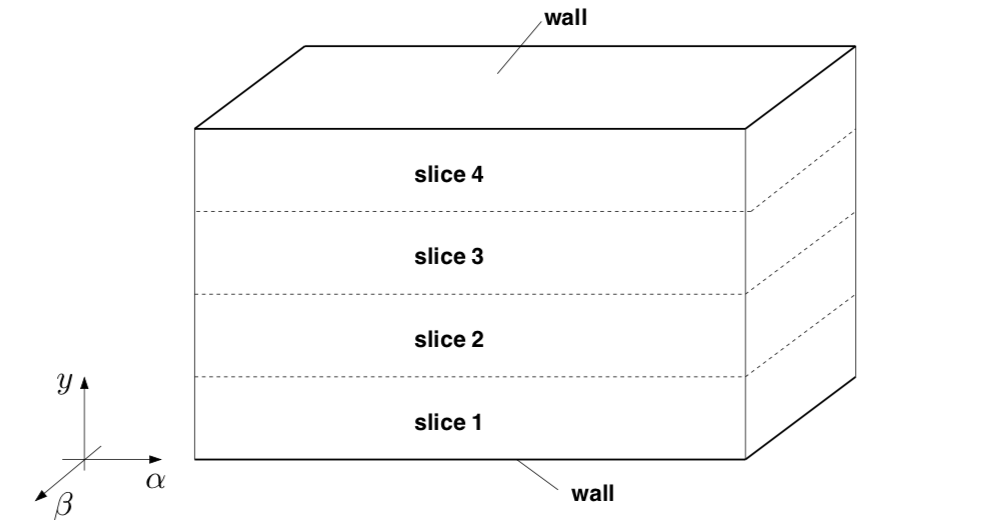
\includegraphics[width=0.8\textwidth]{grafici/decomp_dominio_cpl}
\caption{Original domain decomposition in case of 4 processors}
\label{domain_decomp}
\end{figure}
 allowing to perform convolutions and Fourier transformations locally on each processor, avoiding the cost of non-local transposition for the velocity array and the non-linear terms ones. Such implementation, denominated pipelined-linear-system (PLS), lead to a minimum in communications, in fact this approach require to send and receive only the values stored in the two upper and lower boundary cells of the slice, in order to provide and gather the data required by the fourth-order finite difference scheme, used along the y-direction.
 \par
 Using the PLS approach the bytes exchanged in a three step Range-Kutta method are:
 \begin{equation}
 D_{t} = 3 \times 8 \times (p-1) \frac{3}{2} \times \frac{nx}{p} \frac{nz}{p} \times ny \times 18
 \label{exchange:data:cpl}
 \end{equation}
 where:
 \begin{description}
  \item[3] takes into account the number of time steps;
  \item[8] for counting the bytes;
  \item[$\mathbf{(p-1)}$] is the number of nodes across which the exchange take place;
  \item[ $\mathbf{\frac{3}{2}}$ ] corresponds to the expansion in horizontal modes required by the dealiasing process;
  \item[ $\mathbf{\frac{nx}{p} \times \frac{nz}{p}}$] is the grid portion, for each plane, to exchange with the others nodes;
  \item[18] due to the 3 velocities plus the 6 products to be exchanged twice, before and after the FFT;
  \item[ny] takes into account the number of planes to be exchanged.
\end{description}
Further details about the PLS communications are available in \cite[\nopp chapter 4.2]{cpl:presentazione}. \\
 \par
Although efficient for small processors grid, the performances of this approach falls quickly whether the processors number becomes comparable with \emph{ny}.  Furthermore the communications cost limit the number of parallel process to be just a fraction of the \emph{ny} extension. \\~\\
\par
To avoid such limitations and increase the number of parallel processes we decided to move from PLS approach to something different.
We have identified two possible solutions:
\begin{description}
  \item employ \textbf{slab} decomposition along x or z axis;
  \item employ \textbf{pencil} decomposition.
\end{description}
\begin{figure}
\begin{center}
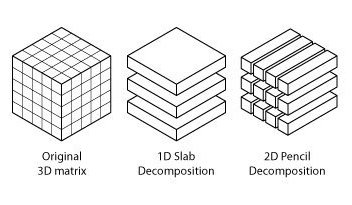
\includegraphics[width=0.7\textwidth]{grafici/decomp_example}
\caption{Kinds of decomposition}
\label{decomposition:example}
\end{center}
\end{figure}
Both implementations require extensive use of the MPI paradigm and, possibly, a library to handle such decompositions.
\par
We opted to employ OpenMPI~\cite{openmpi} for what concern the MPI paradigm, in particular we entrusted to the well established MPI standard 3.1~\cite{MPI:standard}, using OpenMPI release 3.1.3.
The ideas behind the choice of such library rely on the fact that OpenMPI is released behind BSD license, it is designed to group different MPI implementation, avoiding fragmentation and forking problem~\cite{faq:openmpi} and, although less optimized on proprietary fabric such as Intel Omni-Path fabric~\cite{intel:omnipath}\cite{intel:intelmpivsopenmpi}, it is likely the most widespread message passing interface package.
\par
For what concern the decomposition we entrusted in a new library, released by Steven Plimpton from the Sandia National Laboratories, called \emph{fftMPI}~\cite{fftMPI}. Such library leans on the MPI implementation, providing the proper cartesian communicator needed to perform the transposition of the arrays. Next to the communicator, this brand new library provide some useful tweak like permutations or the possibility to select the desired communication mode, which, compared with the FFTW-MPI Transpose~\cite{FFTW05}\cite{FFTW:transpose} features, provide a wider personalization and reduce the work needed for the subsequent operations, such as the FFTs. 
\par
Finally is important to highlight that \emph{fftMPI} can handle both 1D and 2D decomposition, unlike FFTW-MPI.
Others similar libraries are P3DFFT~\cite{p3dfft} from professor Dmitry Pekurovsky (UCSD), PFFT from professor Michael Pippig~\cite{pfft} (Technische Universitat Chemnitz) and 2DECOMP\&FFT~\cite{2decomp} by Ning Li.





\subsection{1D decomposition}
Objective of the decomposition is spread the computational cost across as much as tasks possible. This criteria goes against our needs to have all the dimensions local on chip, in order to carry out the 2D FFT, along $xz$ plane, and to resolve the finite difference scheme, along $y$ direction.
A reasonable tradeoff to these requirements is to employ a slab decomposition. 
\par
Let us focus firstly on the possible approaches to solve the 2D FFTs on $xz$ plane.\par
Given an $N_{x}\times N_{y}\times N_{z}$ grid of points to be distributed over $p$ processors two mainly strategies arise in order to carry out the task and arrange the data as needed.\\
The first approach is to implement a sequence of 2 one-dimensional FFTs, interleaved with data exchange among processors. The other approach, which requires less overall communications, is to make the data local for the dimensions to be transformed (PLS approach~\cite{cpl:presentazione}). \\
\begin{figure}
\begin{center}
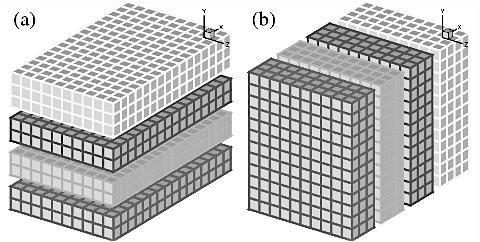
\includegraphics[width=0.6\textwidth]{grafici/1d_decomp}
\caption{Example of 1D decomposition: a) \emph{PLS},  b) \emph{x-slabs}}
\label{1d:decomp}
\end{center}
\end{figure}
\par
Since the code already employed a PLS approach, we moved to the fore ones. In detail we exploit the $N_{y}$ planes independence, to loop among them. Every plane is originally decomposed in $\frac{N_{x}}{p}\times N_{z}$. The code perform the $z$-dimensionals Fourier transformations and an MPI-transposition take place, leading to the new domain decomposition $N_{x} \times \frac{N_{z}}{p}$. In this arrangement the $x$-dimensionals FFTs and subsequent convolutions are performed. Once completed the opposite process takes place. 
\par
At the end of the process we have the velocity convolutions, in Fourier domain, stowed in $yz$ planes. Every plane belong to an independent processor, which, since owns all the $y$ values, can build the RHS term and solve the system.\par
For a tiny cluster or problems with limited dimensions, this kind of approach could be a good choice, since the decomposition limit varies with the lowest decomposed dimension, in this case, $N_{x}$ or $N_{z}$. However the speedup is limited. 
\par
Such limitations about domain decomposition and, consequently, speedups, raise their importance in modern HPC architectures, that counts many thousands cores.  
This limits can be avoided implementing a 2D decomposition.





\subsection{2D decomposition}
In 2D approach the domain is decomposed through a grid of processors, in order to form pencils instead of slabs. The initial pencil dimensions are $\frac{N_{x}}{p_{1}}\times \frac{N_{y}}{p_{2}}\times N_{z}$ where the total amount of task is $p = p_{1}\times p_{2}$.
\par

Starting from such decomposition, we carry out the one-dimensional FFTs along $z$, then we transpose the array in order to have $x$-pencils, so the local dimensions will be $N_{x} \times \frac{N_{y}}{p_{1}} \times \frac{N_{z}}{p_{2}}$. Once here FFTs and convolutions are performed, then we come back to the original decomposition. The final step, needed to guarantee the availability of the values along the $y$ dimension, is to execute a final remap sequence, from the $z$-pencils to $y$-pencils, which will end up with $\frac{N_{x}}{p_{2}} \times N_{y} \times \frac{N_{z}}{p_{1}}$ pencils.

The sequence of operations required to remap a 3D array along the three dimensions is illustrated in figure~\ref{2d:decomp}. 
\par
\begin{figure}
\begin{center}
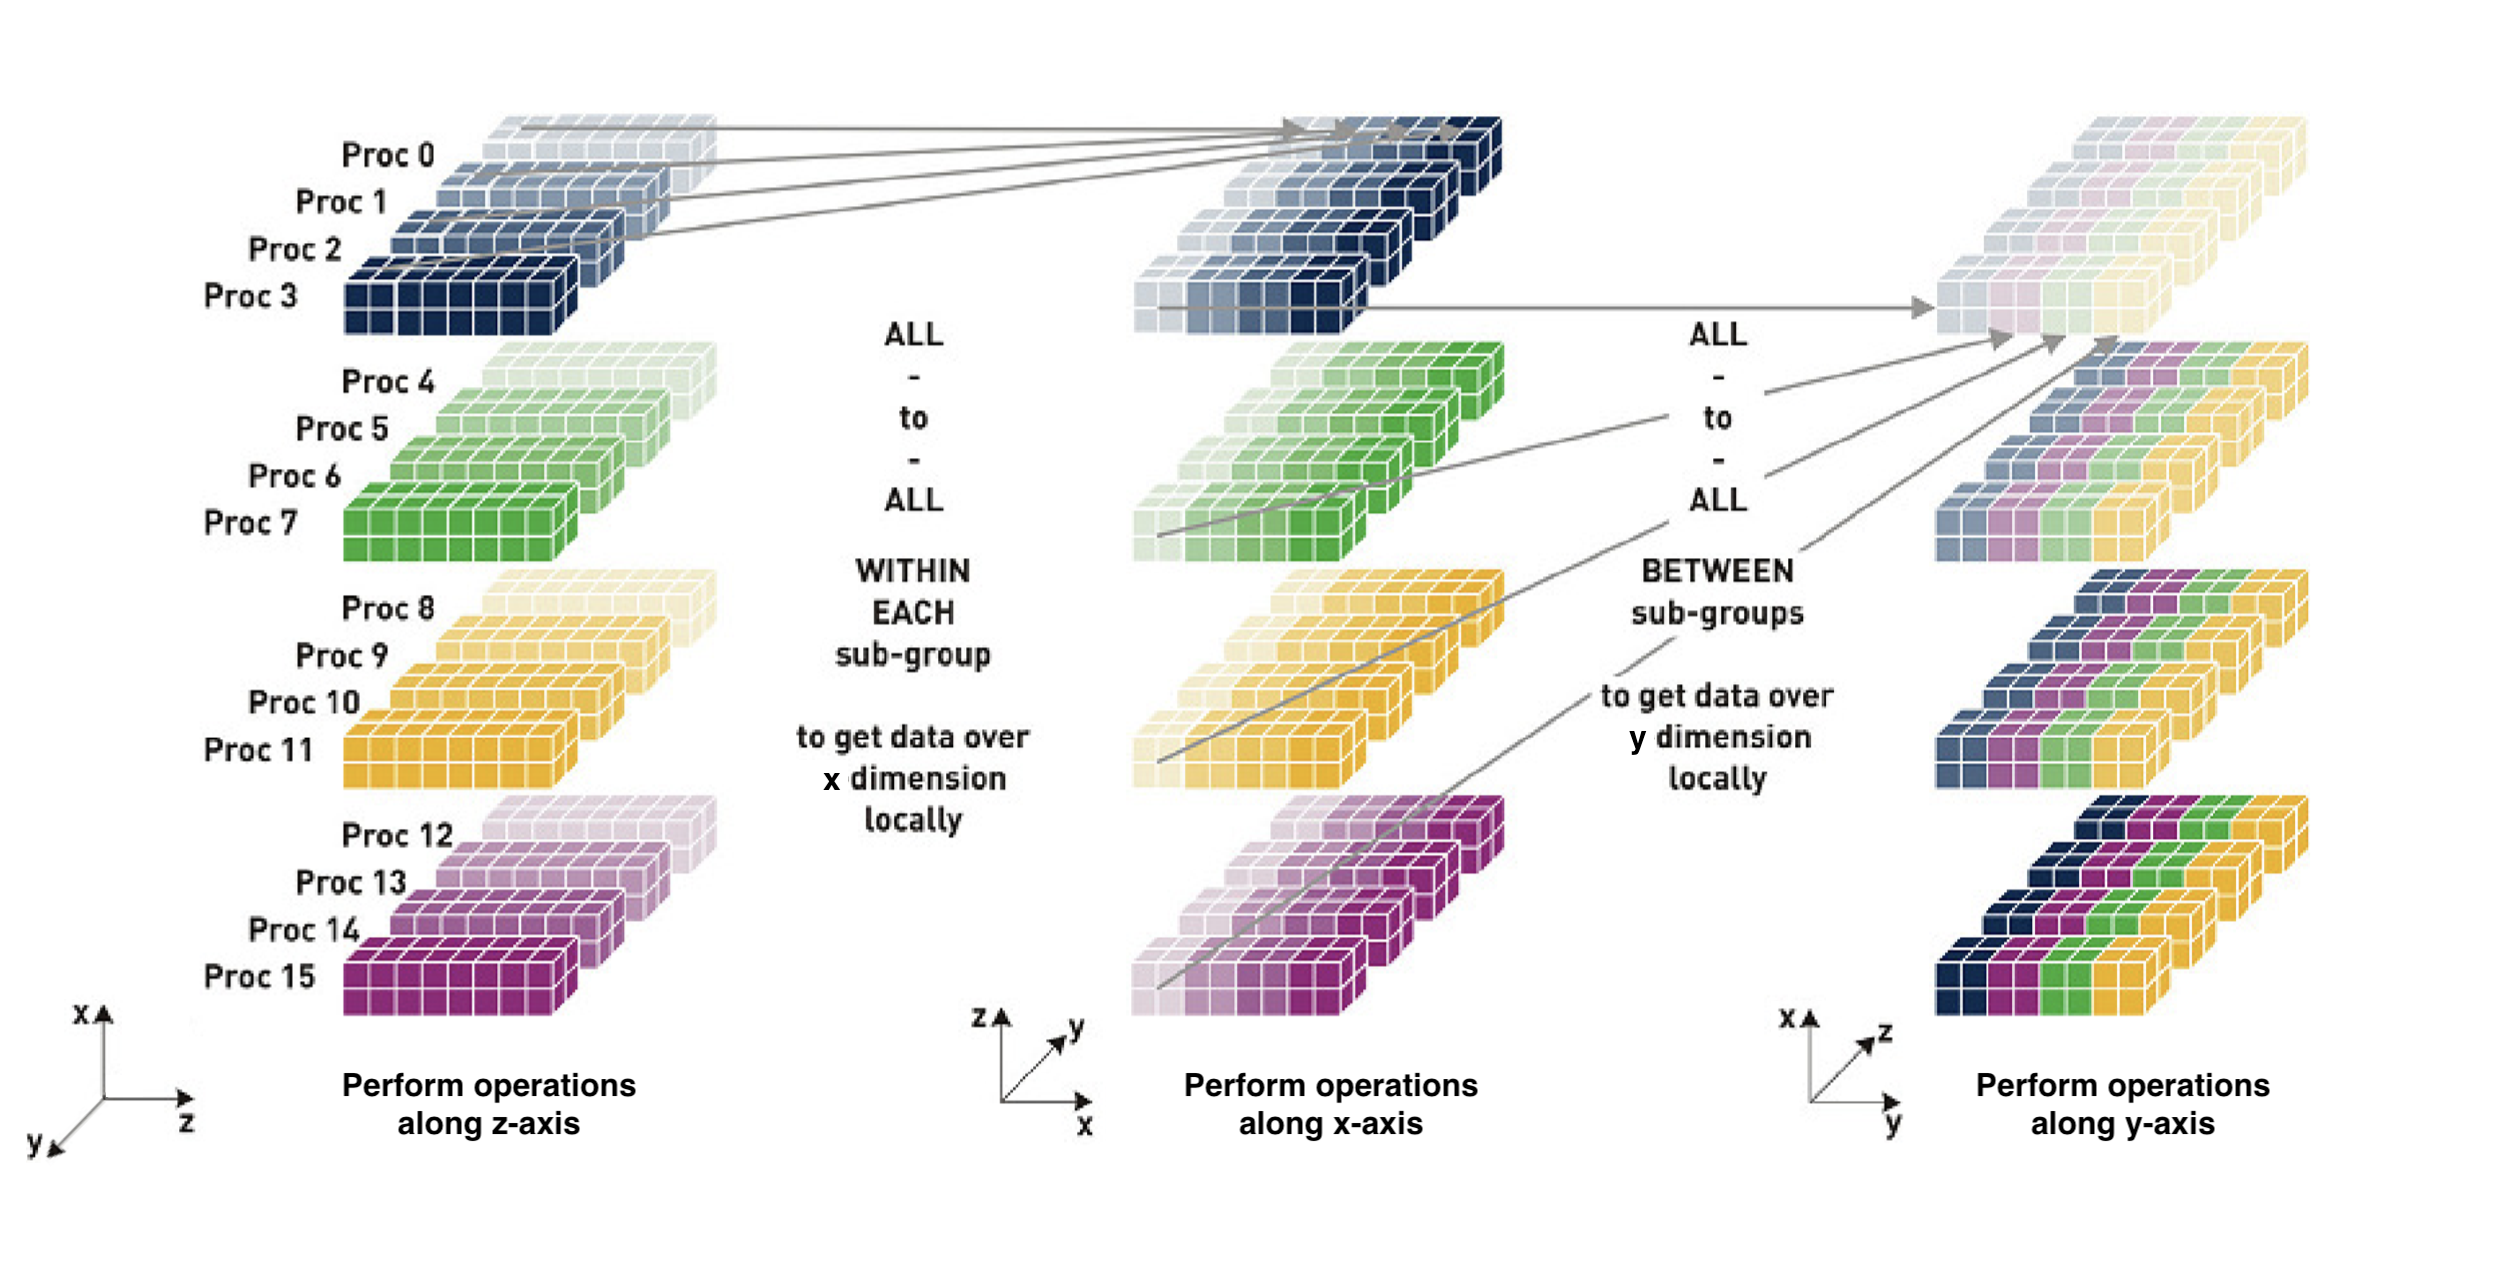
\includegraphics[width=1.08\textwidth]{grafici/2d_decomp}
\caption{2D decomposition of a 3D array}
\label{2d:decomp}
\end{center}
\end{figure}

The 2D approach raise the limit of decomposition to be $N\times N$, allowing to scale to an higher number of processes with respect to the 1D method, thus achieve an higher speedup and efficiency when the dimension of the problem become significant.


\section{Parallel I/O}

Input-output could be a serious bottleneck if we do not pay the right attention.
In particular, when dealing with supercomputers, two major problems arise:
\begin{itemize}
\item needing of parallel I/O,
\item avoid endianness problem related.
\end{itemize}
As first thing let us introduce I/O.\par
\begin{wrapfloat}{figure}{l}{0pt}
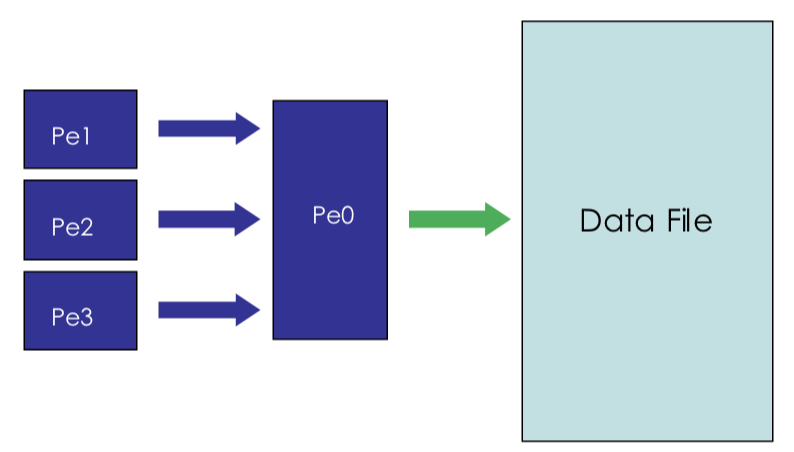
\includegraphics[width=0.5\textwidth]{grafici/masterslave}
\caption{Master-Slaves I/O setup}
\end{wrapfloat}
In computer architecture, the combination of the CPU and main memory, to which the CPU can read or write directly using individual instructions, is considered the brain of a computer. Any transfer of information to or from the CPU/memory combo, for example by reading data from a disk drive, is considered I/O~\cite{io}.
When dealing with cluster the transit of data from disk to CPU is not so straightforward. The presence of multiple CPU require the adoption of one of the following strategies.\par
The most basic strategy is the master-slaves setup. In this kind of strategy a single node of the grid have access to the storage, therefore no scalability is provided. The slave nodes must send/receive data from the master, therefore we face strong slowdown related to the huge workload required to perform I/O by the single node and the following communications among nodes.\par
A second approach is shown here beside and consist in performing distributed I/O on local files. Such kind of implementation is scalable, ensure data consistency and avoid communication during I/O phase. 
\begin{wrapfloat}{figure}{r}{0pt}
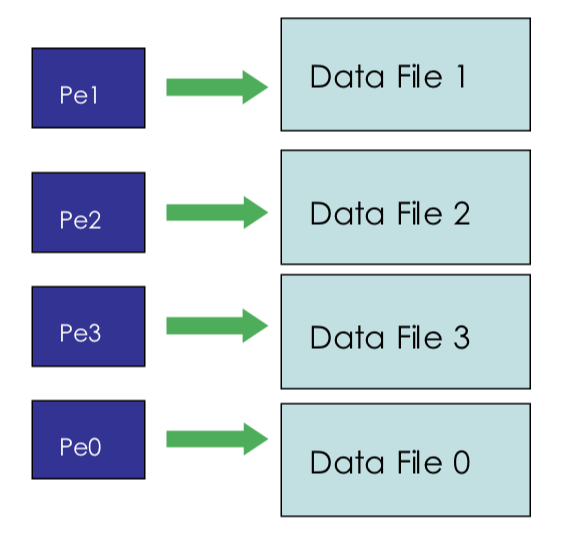
\includegraphics[width=0.5\textwidth]{grafici/localio}
\caption{Distributed I/O on local files}
\end{wrapfloat}However, since every processor writes data on its own hard storage, it require a great deal of post processing work to glue data among each others, which increase linearly with the number of processes. For this reason we can not consider it affordable. \\
\begin{wrapfloat}{figure}{r}{0pt}
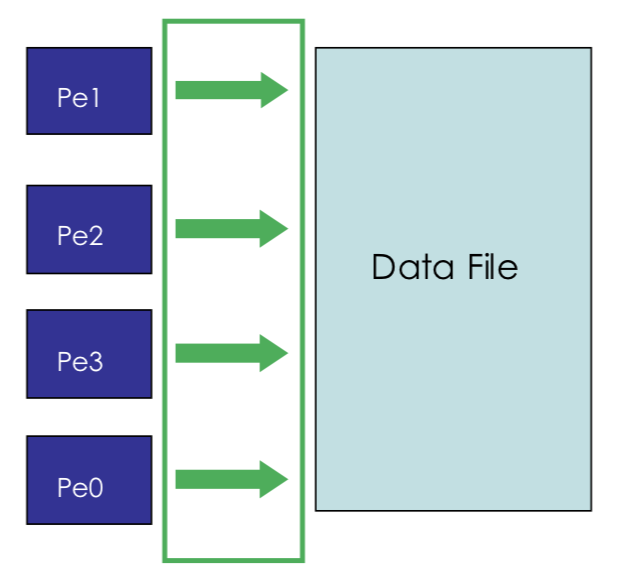
\includegraphics[width=0.5\textwidth]{grafici/mpiio}
\caption{Coordinated controlled accesses}
\end{wrapfloat}
\par
The last kind of I/O setup, which is the most updated and optimized, is the so called coordinated controlled accesses.
Scalability reaches its peak with this kind of implementation, which takes care of possible communications needing by its own.
In this approach every CPU can access to the single storage memory in which the dataset is hosted, and in concomitancy with the other processes, writes the data. As can be understood, the reading/writing operation is intrinsically fragile, since guarantee data consistency can be hard. To avoid consistency lacks, the MPI-IO has been introduced with the deployment of MPI-2 standard~\cite{MPI:standard2}.

On top of MPI-IO several high level I/O libraries arose, two well established examples are parallel netCDF and parallel HDF5. 

At exception of the master-slave approach, every presented strategy require the adoption of a parallel file system.
In computing, a file system or filesystem controls how data is stored and retrieved. Without a file system, information placed in a storage medium would be one large body of data with no way to tell where one piece of information stops and the next begins. By separating the data into pieces and giving each piece a name, the information is easily isolated and identified. We can briefly define the file system as the structure and logic rules used to manage the groups of information and their names.
In the same fashion a parallel file system maintains logical space and provides efficient access to data for distributed memory configurations.\\
\par
Let us establish the concept of endianness.
Intel introduces their white paper with the following sentence:\par
``Endianness describes how multi-byte data is represented by a computer system and is dictated by the CPU architecture of the system. Unfortunately not all computer systems are designed with the same Endian-architecture. The difference in Endian-architecture is an issue when software or data is shared between computer systems''\cite{endianness}.\par
Since our binary database has been built on Marconi, at Cineca, but the post-processing analysis take place on our personal computers, we need to guarantee results portability with a reliable method to store the data. \\
\par
Unfortunately MPI-IO can not set a bit ordering different from the machine's natives ones, and we can not assure portability in this way. To do so we have to move from MPI-IO to a library capable to satisfy our requirements.\par
Employ the well established parallel HDF5 library is the natural choice.





\section{Third party libraries}
\subsection{fftMPI}
\emph{fftMPI} is the package we choose to implement to take care of the decomposition. It is installed through the classic set of commands 
\begin{lstlisting}
./configure 
make 
make install
\end{lstlisting}
and produce a couple of different libraries, once for 1D and once for 2D decomposition.
\par
These libraries are accessed through four headers, based on the user needing. In our case we were interested at the remap APIs for 3D arrays, so we called 
\begin{lstlisting} 
remap3d.h .
\end{lstlisting}
Once the header was included we compiled the source code with 
\begin{lstlisting}
-lfft3dmpi
\end{lstlisting}
flag to produce the executable. To link the code is mandatory to use 
\begin{lstlisting}
mpicxx
\end{lstlisting}
or equivalent, since \emph{fftMPI} is written in C++, and not in C. \\
\par
Currently the remap works with floating point data only. Anyway, each datum in a distributed 3D grid can be one or more floating point values. In our case, we employed the method with the parameter
\begin{lstlisting}
nqty = 2
\end{lstlisting}
so that the method select two adjacent floating point values per grid point, and treat them as a single complex number. \\
\par
A pseudo-code of such package expect the following structure:
\begin{lstlisting}
#include "remap3d_wrap.h" 
remap3d_create(MPI_COMM_WORLD,&remap);

remap3d_set(remap,"collective",cflag);
remap3d_set(remap,"pack",pflag);
remap3d_set(remap,"memory",mflag); 

remap3d_setup(local_input_tiles_coords, local_output_tiles_coords,
              nqty,permute,memoryflag,&sendsize,&recvsize); 
              
FFT_SCALAR *ARR = (FFT_SCALAR *) malloc(remapsize*sizeof(FFT_SCALAR));
FFT_SCALAR *sendbuf = (FFT_SCALAR *) malloc(sendsize*sizeof(FFT_SCALAR));
FFT_SCALAR *recvbuf = (FFT_SCALAR *) malloc(recvsize*sizeof(FFT_SCALAR)); 

/* Fill the array ARR with data */
ARR= ...

remap3d_remap(remap,ARR,ARR,sendbuf,recvbuf); 

remap3d_destroy(remap); 
\end{lstlisting}
As we can see the process is made up of:
\begin{itemize}
\item create the remap container;
\item set options for the remap;
\item define the tiles dimensions and commit the container;
\item execute the remap;
\item destroy the remap container.
\end{itemize}
\par
The options allow users to set the method, used by MPI, to pass the messages. For example, it is possible to decide whether to use collective calls instead of point-to-point communications, or it is possible to select how to pack the messages before sending them.
\par
For further informations, and the source code,\cite{fftMPI}.


\subsection{Parallel HDF5 Library}
Hierarchical Data Format 5, or HDF5~\cite{hdf5}, is widespread scientific data format used by many application to deal with large sets of data. Parallel Hierarchical Data Format 5, or pHDF5, is the parallelized version for clusters.\par
Designed to store and organize large amounts of data, HDF5 has been originally developed at the National Center for Supercomputing Applications. 
The crucial feature is its ability to store binary dataset in a processor independent fashion, guaranteeing the portability of the data. This allows extremely compact file dimensions, since we are dealing with binary data, and in the same time we can exploit the advantages of ASCII encoding.\par
We could think at the a parallel I/O as a bridge between the application and the data, which are stored on memory. In this parallelism our high-level library can be thought as the deck of the bridge. Such deck is built on top of pylons, which is the middleware, the MPI-IO. Our library provide an high level of abstractions, allowing to instruct and tune the middleware to perform the requested operations. On its own the MPI-IO deals with organizing access by many processes. Everything is anchored to the ground through foundations, which is our parallel file system.\par
The hierarchical file ordering allows to define a Linux like environment made up of root folder, subfolders, tables, figure, attributes, links and others useful things to maintain the database as readable as possible.\par
\begin{figure}
\begin{center}
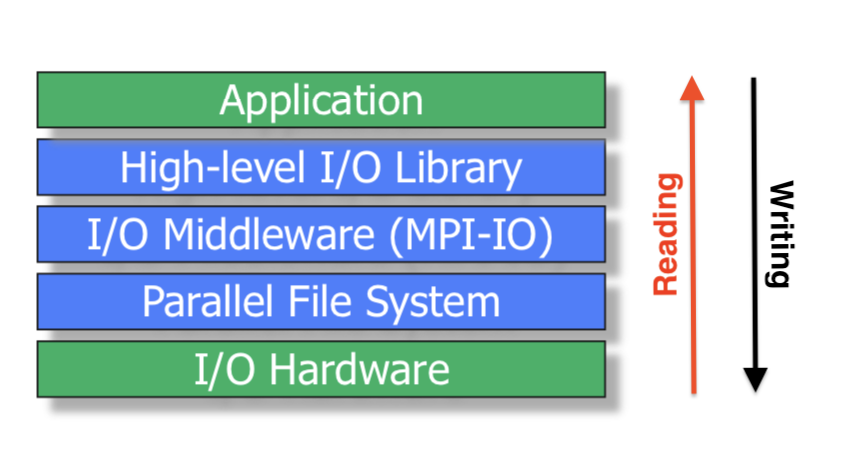
\includegraphics[scale=0.4]{grafici/parallelio}
\caption{Ideal structure of a parallel I/O implementation}
\label{default}
\end{center}
\end{figure}

The price for the high flexibility of such data format is the impossibility to have a plug and play VTK reader. In fact we have to rely on third party software to instruct the VTK tool, in our case Paraview, to inspect the database. \par
We decide to use XDMF3~\cite{xdmf3}, acronym of eXtensible Data Model and Format~3, to generate an XML file to put beside of our HDF5 file, so that Paraview, or any other VTK software, use to read the database.
Such XML file is automatically generated when the post processor is run. It contains the environmental conditions, such as domain geometry, cell placement, timestep and some instruction to join the velocities data of a cell into a vector. It is used to tell to the VTK reader where and what read from the HDF5 file.

